% Practice Test 05 — Texas Edition
% Questions: 30 (25 MC + 5 SA)
% Generated by scripts/generate_practice_tests.py

\begin{practiceQuestion}{1-3-q04}{mc}
\begin{questionText}
Bananas cost a fixed price per pound. The table shows the relationship. What is $k$?

\begin{center}
\begin{tabular}{|c|c|}
\hline \textbf{Pounds} & \textbf{Cost (\$)} \\ \hline $2$ & $\$1.30$ \\ $5$ & $\$3.25$ \\ $8$ & $\$5.20$ \\ \hline
\end{tabular}
\end{center}
\end{questionText}
\choiceA{$\$0.55$ per pound}
\choiceB{$\$0.65$ per pound}
\choiceC{$\$1.30$ per pound}
\choiceD{$\$1.54$ per pound}
\correctAnswer{B}
\explanation{$k = \frac{1.30}{2} = 0.65$. Check: $\frac{3.25}{5} = 0.65$ and $\frac{5.20}{8} = 0.65$. Bananas cost $\$0.65$ per pound.}
\end{practiceQuestion}

\begin{practiceQuestion}{1-6-q15}{mc}
\begin{questionText}
A car uses $3$ gallons of gas every $87$ miles. How many gallons does it need for a $435$-mile trip?
\end{questionText}
\choiceA{$10$}
\choiceB{$12$}
\choiceC{$15$}
\choiceD{$18$}
\correctAnswer{C}
\explanation{$\frac{3}{87} = \frac{x}{435}$. Cross-multiply: $87x = 1{,}305$, so $x = 15$ gallons.}
\end{practiceQuestion}

\begin{practiceQuestion}{2-1-q06}{mc}
\begin{questionText}
$14$ is what percent of $56$?
\end{questionText}
\choiceA{$14\%$}
\choiceB{$20\%$}
\choiceC{$25\%$}
\choiceD{$28\%$}
\correctAnswer{C}
\explanation{Divide the part by the whole: $14 \div 56 = 0.25 = 25\%$.}
\end{practiceQuestion}

\begin{practiceQuestion}{2-3-q24}{sa}
\begin{questionText}
A town's population increased by $8\%$ from $25{,}000$. What is the new population?
\end{questionText}
\correctAnswer{$27{,}000$}
\explanation{$25{,}000 \times 1.08 = 27{,}000$.}
\end{practiceQuestion}

\begin{practiceQuestion}{2-6-q27}{gmc}
\begin{questionText}
The table below compares two savings plans. Which plan earns more interest?

\begin{center}
\begin{tabular}{|l|c|c|c|}
\hline
 & \textbf{Principal} & \textbf{Rate} & \textbf{Time} \\
\hline
Plan A & $\$2{,}000$ & $3\%$ & $4$ years \\
\hline
Plan B & $\$1{,}500$ & $4\%$ & $4$ years \\
\hline
\end{tabular}
\end{center}
\end{questionText}
\choiceA{Plan A by $\$240$}
\choiceB{Plan A by $\$0$}
\choiceC{Plan B by $\$240$}
\choiceD{They earn the same}
\correctAnswer{D}
\explanation{Plan A: $2{,}000 \times 0.03 \times 4 = \$240$. Plan B: $1{,}500 \times 0.04 \times 4 = \$240$. Both earn $\$240$.}
\end{practiceQuestion}

\begin{practiceQuestion}{2-8-q16}{mc}
\begin{questionText}
Which payment method does NOT involve borrowing money?
\end{questionText}
\choiceA{Credit card}
\choiceB{Loan from a bank}
\choiceC{Debit card}
\choiceD{Line of credit}
\correctAnswer{C}
\explanation{A debit card uses money you already have. The other options all involve borrowing money.}
\end{practiceQuestion}

\begin{practiceQuestion}{2-9-q10}{mc}
\begin{questionText}
Experts suggest saving at least what percent of your income?
\end{questionText}
\choiceA{$1\%$}
\choiceB{$5\%$}
\choiceC{$10\%$}
\choiceD{$50\%$}
\correctAnswer{C}
\explanation{Financial experts generally recommend saving at least $10\%$ of income.}
\end{practiceQuestion}

\begin{practiceQuestion}{2-10-q28}{gmc}
\begin{questionText}
The table compares simple and compound interest on $\$200$ at $10\%$ for $3$ years. What is the compound interest total after Year $3$?

\begin{center}
\begin{tabular}{|c|c|c|}
\hline
\textbf{Year} & \textbf{Simple} & \textbf{Compound} \\
\hline
$0$ & $\$200$ & $\$200$ \\
\hline
$1$ & $\$220$ & $\$220$ \\
\hline
$2$ & $\$240$ & $\$242$ \\
\hline
$3$ & $\$260$ & ? \\
\hline
\end{tabular}
\end{center}
\end{questionText}
\choiceA{$\$260$}
\choiceB{$\$264$}
\choiceC{$\$266.20$}
\choiceD{$\$268$}
\correctAnswer{C}
\explanation{Year 3 compound: $242 \times 1.10 = \$266.20$.}
\end{practiceQuestion}

\begin{practiceQuestion}{4-1-q13}{mc}
\begin{questionText}
A rectangle has length $2x + 3$ and width $4$. Which expression gives its perimeter?
\end{questionText}
\choiceA{$8x + 12$}
\choiceB{$2x + 7$}
\choiceC{$4x + 14$}
\choiceD{$8x + 6$}
\correctAnswer{C}
\explanation{Perimeter $= 2(\text{length} + \text{width}) = 2(2x + 3 + 4) = 2(2x + 7) = 4x + 14$.}
\end{practiceQuestion}

\begin{practiceQuestion}{4-2-q01}{mc}
\begin{questionText}
Which pair of terms are like terms?
\end{questionText}
\choiceA{$3x$ and $3y$}
\choiceB{$5m$ and $-2m$}
\choiceC{$4n$ and $4n^2$}
\choiceD{$7$ and $7x$}
\correctAnswer{B}
\explanation{Like terms have the same variable raised to the same power. $5m$ and $-2m$ both have the variable $m$ to the first power.}
\end{practiceQuestion}

\begin{practiceQuestion}{5-3-q03}{mc}
\begin{questionText}
What is the first step to solve $5(x + 2) = 35$ using the ``divide first'' method?
\end{questionText}
\choiceA{Subtract $2$ from both sides}
\choiceB{Distribute $5$ to get $5x + 10 = 35$}
\choiceC{Divide both sides by $5$}
\choiceD{Subtract $5$ from both sides}
\correctAnswer{C}
\explanation{The ``divide first'' method divides both sides by $5$: $x + 2 = 7$.}
\end{practiceQuestion}

\begin{practiceQuestion}{5-4-q08}{mc}
\begin{questionText}
A recipe calls for $\dfrac{3}{4}$ cup of sugar per batch. You already used $\dfrac{1}{2}$ cup. You have $2\dfrac{3}{4}$ cups total. The equation $\dfrac{3}{4}b + \dfrac{1}{2} = 2\dfrac{3}{4}$ finds how many more batches $b$ you can make. What is $b$?
\end{questionText}
\choiceA{$b = 3$}
\choiceB{$b = 4$}
\choiceC{$b = 2$}
\choiceD{$b = 3\dfrac{2}{3}$}
\correctAnswer{A}
\explanation{Subtract $\frac{1}{2}$: $\frac{3}{4}b = 2\frac{1}{4} = \frac{9}{4}$. Multiply by $\frac{4}{3}$: $b = \frac{9}{4} \times \frac{4}{3} = 3$.}
\end{practiceQuestion}

\begin{practiceQuestion}{5-5-q18}{mc}
\begin{questionText}
Solve $-x + 9 \leq 15$.
\end{questionText}
\choiceA{$x \leq -6$}
\choiceB{$x \geq 6$}
\choiceC{$x \geq -6$}
\choiceD{$x \leq 6$}
\correctAnswer{C}
\explanation{Subtract $9$: $-x \leq 6$. Multiply by $-1$ and flip: $x \geq -6$.}
\end{practiceQuestion}

\begin{practiceQuestion}{5-6-q29}{gsa}
\begin{questionText}
Solve $-3x + 9 > 0$. Then graph the solution on the number line below by describing the circle type and shading direction.

\begin{center}
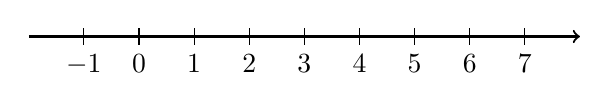
\begin{tikzpicture}[scale=0.7]
  \draw[thick,->] (-2,0) -- (8,0);
  \foreach \x in {-1,...,7} \draw (\x,0.15) -- (\x,-0.15) node[below] {$\x$};
\end{tikzpicture}
\end{center}
\end{questionText}
\correctAnswer{$x < 3$; open circle at $3$, shade left}
\explanation{Subtract $9$: $-3x > -9$. Divide by $-3$ and flip: $x < 3$. Open circle at $3$, shade left.}
\end{practiceQuestion}

\begin{practiceQuestion}{6-2-q17}{mc}
\begin{questionText}
A map uses $1$ cm $= 60$ km. You redraw it at $1$ cm $= 20$ km. A triangle on the original has an area of $4$ cm$^2$. What is its area on the new map?
\end{questionText}
\choiceA{$12$ cm$^2$}
\choiceB{$16$ cm$^2$}
\choiceC{$36$ cm$^2$}
\choiceD{$48$ cm$^2$}
\correctAnswer{C}
\explanation{Scale ratio: $\frac{60}{20} = 3$. Area scales by $3^2 = 9$. New area: $4 \times 9 = 36$ cm$^2$.}
\end{practiceQuestion}

\begin{practiceQuestion}{6-3-q08}{mc}
\begin{questionText}
Which set of conditions produces exactly one triangle?
\end{questionText}
\choiceA{Three angles: $40°$, $60°$, $80°$}
\choiceB{One side: $5$ cm}
\choiceC{Three sides: $3$ cm, $5$ cm, $7$ cm}
\choiceD{Two sides: $4$ cm and $6$ cm}
\correctAnswer{C}
\explanation{Three valid side lengths (SSS) with the triangle inequality satisfied produce exactly one unique triangle. AAA gives many, and knowing only one or two side lengths is not enough.}
\end{practiceQuestion}

\begin{practiceQuestion}{6-4-q08}{mc}
\begin{questionText}
You know two angles ($50°$ and $70°$) and the side between them is $8$ cm. What triangle condition is this?
\end{questionText}
\choiceA{SSS}
\choiceB{SAS}
\choiceC{ASA}
\choiceD{AAS}
\correctAnswer{C}
\explanation{Two angles and the included side is the ASA (Angle-Side-Angle) condition.}
\end{practiceQuestion}

\begin{practiceQuestion}{6-5-q25}{sa}
\begin{questionText}
A square pyramid has a base edge of $8$ cm. It is sliced parallel to the base halfway up. Is the cross-section larger, smaller, or the same size as the base?
\end{questionText}
\correctAnswer{Smaller than the base}
\explanation{A horizontal cut parallel to the base of a pyramid produces a similar shape that is smaller than the base. Halfway up, the cross-section is a $4$ cm square (half the edge length).}
\end{practiceQuestion}

\begin{practiceQuestion}{6-8-q02}{mc}
\begin{questionText}
Two similar rectangles have corresponding sides $5$ cm and $15$ cm. If the shorter rectangle has a width of $3$ cm, what is the width of the larger rectangle?
\end{questionText}
\choiceA{$6$ cm}
\choiceB{$9$ cm}
\choiceC{$13$ cm}
\choiceD{$45$ cm}
\correctAnswer{B}
\explanation{Scale factor: $\frac{15}{5} = 3$. Width of larger: $3 \times 3 = 9$ cm.}
\end{practiceQuestion}

\begin{practiceQuestion}{7-4-q10}{mc}
\begin{questionText}
A figure is made of a trapezoid with parallel sides $6$ cm and $10$ cm, and height $4$ cm. Which expression gives its area?
\end{questionText}
\choiceA{$6 \times 10 \times 4$}
\choiceB{$\frac{1}{2} \times 6 \times 10$}
\choiceC{$\frac{1}{2} \times (6 + 10) \times 4$}
\choiceD{$(6 + 10) \times 4$}
\correctAnswer{C}
\explanation{Area of a trapezoid $= \frac{1}{2}(b_1 + b_2) \times h = \frac{1}{2}(6 + 10) \times 4 = 32$ cm$^2$.}
\end{practiceQuestion}

\begin{practiceQuestion}{7-5-q10}{mc}
\begin{questionText}
A cube has a surface area of $54$ cm$^2$. What is the area of one face?
\end{questionText}
\choiceA{$6$ cm$^2$}
\choiceB{$9$ cm$^2$}
\choiceC{$18$ cm$^2$}
\choiceD{$27$ cm$^2$}
\correctAnswer{B}
\explanation{A cube has $6$ identical faces. Area of one face $= 54 \div 6 = 9$ cm$^2$.}
\end{practiceQuestion}

\begin{practiceQuestion}{7-6-q18}{mc}
\begin{questionText}
A trapezoidal prism has a trapezoidal base with parallel sides $4$ cm and $6$ cm, height $3$ cm, and the prism length is $10$ cm. What is its volume?
\end{questionText}
\choiceA{$60$ cm$^3$}
\choiceB{$120$ cm$^3$}
\choiceC{$150$ cm$^3$}
\choiceD{$180$ cm$^3$}
\correctAnswer{C}
\explanation{$B = \frac{1}{2}(4 + 6) \times 3 = 15$ cm$^2$. $V = 15 \times 10 = 150$ cm$^3$.}
\end{practiceQuestion}

\begin{practiceQuestion}{8-1-q11}{mc}
\begin{questionText}
A survey of $200$ randomly selected adults found that $60\%$ prefer coffee over tea. If the city has $50{,}000$ adults, about how many prefer coffee?
\end{questionText}
\choiceA{$12{,}000$}
\choiceB{$20{,}000$}
\choiceC{$30{,}000$}
\choiceD{$60{,}000$}
\correctAnswer{C}
\explanation{$60\%$ of $50{,}000 = 0.60 \times 50{,}000 = 30{,}000$.}
\end{practiceQuestion}

\begin{practiceQuestion}{8-2-q08}{mc}
\begin{questionText}
A sample of $60$ bags of chips has a mean weight of $28.5$ grams. The label says $30$ grams. What can you infer?
\end{questionText}
\choiceA{All bags weigh exactly $30$ grams}
\choiceB{The bags may be slightly underweight on average}
\choiceC{The sample is too small to make any conclusion}
\choiceD{The label is definitely wrong}
\correctAnswer{B}
\explanation{The sample mean ($28.5$ g) is below the labeled weight ($30$ g), suggesting bags may be slightly underweight on average.}
\end{practiceQuestion}

\begin{practiceQuestion}{8-4-q30}{gsa}
\begin{questionText}
The table shows test scores for two science classes.

\begin{center}
\begin{tabular}{|l|c|c|c|c|c|c|c|c|c|c|}
\hline
\textbf{Class A} & $60$ & $65$ & $70$ & $75$ & $80$ & $85$ & $90$ & $95$ & & \\
\hline
\textbf{Class B} & $72$ & $74$ & $76$ & $78$ & $80$ & $82$ & $84$ & $86$ & & \\
\hline
\end{tabular}
\end{center}

Find the mean, median, and range for each class. Which class performed more consistently?
\end{questionText}
\correctAnswer{Both means $= 77.5$; both medians $= 77.5$; Class A range $= 35$, Class B range $= 14$. Class B is more consistent.}
\explanation{Class A: mean $= \frac{620}{8} = 77.5$, median $= \frac{75+80}{2} = 77.5$, range $= 95 - 60 = 35$. Class B: mean $= \frac{632}{8} = 79$, median $= \frac{78+80}{2} = 79$, range $= 86 - 72 = 14$. Class B has a much smaller range, so its scores are more consistent.}
\end{practiceQuestion}

\begin{practiceQuestion}{8-5-q02}{mc}
\begin{questionText}
Which of the following is true about the leaves in a stem-and-leaf plot?
\end{questionText}
\choiceA{Leaves are listed in random order}
\choiceB{Leaves are listed in order from least to greatest}
\choiceC{Each leaf represents the tens digit}
\choiceD{Leaves are always single digits from $1$ to $9$}
\correctAnswer{B}
\explanation{Leaves must be arranged in order from least to greatest so the data is easy to read.}
\end{practiceQuestion}

\begin{practiceQuestion}{8-6-q26}{gmc}
\begin{questionText}
The circle graph shows how $400$ students get to school.

\begin{center}
\begin{tikzpicture}[scale=1.2]
  % Bus 40%, Walk 25%, Car 20%, Bike 15%
  \fill[funBlue!60] (0,0) -- (0,1.5) arc (90:90-144:1.5) -- cycle;
  \fill[funGreen!60] (0,0) -- (90-144:1.5) arc (90-144:90-144-90:1.5) -- cycle;
  \fill[funOrange!60] (0,0) -- (90-144-90:1.5) arc (90-144-90:90-144-90-72:1.5) -- cycle;
  \fill[funRed!40] (0,0) -- (90-144-90-72:1.5) arc (90-144-90-72:90:1.5) -- cycle;
  \draw (0,0) circle (1.5);
  \node[font=\small\bfseries] at (60:1) {Bus};
  \node[font=\tiny] at (60:0.65) {$40\%$};
  \node[font=\small\bfseries] at (-30:1) {Walk};
  \node[font=\tiny] at (-30:0.65) {$25\%$};
  \node[font=\small\bfseries] at (-110:1) {Car};
  \node[font=\tiny] at (-110:0.65) {$20\%$};
  \node[font=\small\bfseries] at (170:1) {Bike};
  \node[font=\tiny] at (170:0.65) {$15\%$};
\end{tikzpicture}
\end{center}

How many students walk to school?
\end{questionText}
\choiceA{$25$}
\choiceB{$60$}
\choiceC{$80$}
\choiceD{$100$}
\correctAnswer{D}
\explanation{$25\%$ of $400 = 0.25 \times 400 = 100$ students.}
\end{practiceQuestion}

\begin{practiceQuestion}{9-4-q24}{sa}
\begin{questionText}
Create a non-uniform probability model for a spinner with $3$ sections (A, B, C) where A is twice as likely as B, and C has the same probability as B. Write the probability of each section.
\end{questionText}
\correctAnswer{$P(A) = \frac{1}{2}$, $P(B) = \frac{1}{4}$, $P(C) = \frac{1}{4}$}
\explanation{Let $P(B) = x$. Then $P(A) = 2x$ and $P(C) = x$. Total: $2x + x + x = 4x = 1$, so $x = \frac{1}{4}$. $P(A) = \frac{1}{2}$, $P(B) = P(C) = \frac{1}{4}$.}
\end{practiceQuestion}

\begin{practiceQuestion}{9-6-q13}{mc}
\begin{questionText}
Two coins are flipped. What is the probability of getting at least one head?
\end{questionText}
\choiceA{$\frac{1}{4}$}
\choiceB{$\frac{1}{2}$}
\choiceC{$\frac{3}{4}$}
\choiceD{$1$}
\correctAnswer{C}
\explanation{At least one head: HH, HT, TH — that is $3$ out of $4$. $P = \frac{3}{4}$. Or: $1 - P(\text{no heads}) = 1 - \frac{1}{4} = \frac{3}{4}$.}
\end{practiceQuestion}

\begin{practiceQuestion}{9-7-q11}{mc}
\begin{questionText}
A bag has $3$ red and $7$ blue marbles. To simulate drawing one marble, you could use random digits $0$--$9$. Which digits would represent red?
\end{questionText}
\choiceA{$0, 1, 2$}
\choiceB{$0, 1, 2, 3$}
\choiceC{$0, 1, 2, 3, 4, 5, 6$}
\choiceD{$7, 8, 9$}
\correctAnswer{A}
\explanation{Red has a $\frac{3}{10}$ probability. Using $3$ digits ($0, 1, 2$) out of $10$ gives $\frac{3}{10} = 30\%$.}
\end{practiceQuestion}
